\documentclass[11pt,a4paper,twoside,openright]{report}
\usepackage[utf8]{inputenc}

\usepackage[]{feupteses}
%\usepackage[square,sort,comma,numbers]{natbib}


\usepackage[english]{babel}


%\bibliographystyle{IEEEtran}

%\usepackage[square]{natbib}
\usepackage{graphicx}
\usepackage{framed}
\usepackage{multirow}
\usepackage{lipsum}  
\usepackage{verbatim}
\usepackage{amsmath}
\usepackage{longtable}
\usepackage{caption}
\usepackage{subcaption}


\usepackage{array}
\usepackage{adjustbox}


%\usepackage[oneside,width=17.5cm,height=24cm,left=2cm]{geometry}
%\usepackage[nolist,nohyperlinks]{acronym}

\usepackage[]{nomencl}
\usepackage[final]{pdfpages}

%\usepackage{biblatex}
%\addbibresource{references.bib}



\newcolumntype{L}[1]{>{\raggedright\let\newline\\\arraybackslash\hspace{0pt}}m{#1}}
\newcolumntype{C}[1]{>{\centering\let\newline\\\arraybackslash\hspace{0pt}}m{#1}}
\newcolumntype{R}[1]{>{\raggedleft\let\newline\\\arraybackslash\hspace{0pt}}m{#1}}

%%%  para ter capítulos xpto
%%%  https://hstuart.dk/2007/05/21/styling-the-chapter/


\usepackage{tikz, blindtext}
\usepackage{kpfonts}
\usepackage[explicit]{titlesec}
\usepackage{xcolor}
\definecolor{FEUP_color}{RGB}{140,45,25}

\newcommand*\chapterlabel{}
\titleformat{\chapter}
{\gdef\chapterlabel{}
	\normalfont\sffamily\huge\bfseries\scshape}
{\gdef\chapterlabel{\thechapter\ }}{0pt}
{\begin{tikzpicture}[remember picture,overlay]
	\node[yshift=-6cm] at (current page.north west)
	{\begin{tikzpicture}[remember picture, overlay]
		%\draw[fill=white] (-1,0) rectangle
	%	(1.2\paperwidth,8cm);
		\node[anchor=west,xshift=3cm,rectangle,
		rounded corners=1pt,inner sep=11pt,
		fill=black]
		{\color{white}\chapterlabel#1};
		\end{tikzpicture}
	};
\end{tikzpicture}
}
\titlespacing*{\chapter}{0pt}{50pt}{50pt}

\makenomenclature
\nomenclature{\textbf{AMI}}{Advanced Metering Infrastructure }
\nomenclature{\textbf{EMS}}{Energy Management System}
\nomenclature{\textbf{EIS}}{Energy Information Systems}
\nomenclature{\textbf{SG}}{Smart Grid}
\nomenclature{\textbf{IT}}{Information Technology}
\nomenclature{\textbf{AMR}}{Automatic Meter Readers}
\nomenclature{\textbf{SM}}{Smart Meter}
\nomenclature{\textbf{IEC}}{International Electrotechnical Commission}
\nomenclature{\textbf{EC}}{European Commission}
\nomenclature{\textbf{EU}}{European Union}
\nomenclature{\textbf{EGs}}{Expert Groups}
\nomenclature{\textbf{TSOs}}{Transmission System Operators}
\nomenclature{\textbf{DSOs}}{Distribution System Operators}
\nomenclature{\textbf{DNOs}}{Distribution Network Operators}

%2.2 to 2.6

\nomenclature{\textbf{WAN}}{Wide Area Network}
\nomenclature{\textbf{NAN}}{Neighborhood Area Network}
\nomenclature{\textbf{LAN}}{Local Area Network}
\nomenclature{\textbf{HAN}}{Home Area Network}
\nomenclature{\textbf{MAN}}{Metropolitan Area Network}
\nomenclature{\textbf{PEVs}}{Plug-in Electric Vehicles}
\nomenclature{\textbf{IHD}}{In-Home Displays}
\nomenclature{\textbf{MDMS}}{Meter Data Management System}
\nomenclature{\textbf{DR}}{Demand-Response}
\nomenclature{\textbf{SEIS}}{Smart Energy Management Systems}
\nomenclature{\textbf{ICT}}{Information and Communication Technologies}
\nomenclature{\textbf{O\&M}}{Operation and Management}
\nomenclature{\textbf{S2R}}{Shift2Rail program}
\nomenclature{\textbf{IP3}}{Innovation Programme 3 (of Shift2Rail)}
\nomenclature{\textbf{ODM}}{Operational Data Management}
\nomenclature{\textbf{UA}}{User Applications}
\nomenclature{\textbf{RDERMS}}{Railway dedicated Distributed Energy Resource Management System}

%chapter 3

\nomenclature{\textbf{SCADA}}{Supervisory Control and Data Acquisition}
\nomenclature{\textbf{PLC}}{Power Line Communication}
\nomenclature{\textbf{DCM}}{Data Collection Mechanism}
\nomenclature{\textbf{ADSL}}{Asymmetric  Digital  Subscriber  Line}
\nomenclature{\textbf{GSM}}{Global Systems Network}

\nomenclature{\textbf{SMS}}{Short Message Service}
\nomenclature{\textbf{CDMA}}{Code Division Multiple Access}
\nomenclature{\textbf{D-AMPS}}{Digital Advanced Mobile Phone Service}
\nomenclature{\textbf{RF}}{Radio Frequency}
\nomenclature{\textbf{WLAN}}{Wireless Local Area Network}
\nomenclature{\textbf{GPRS}}{General Packet Radio Service}
\nomenclature{\textbf{WiMAX}}{Worldwide Interoperability for Microwave Access}
\nomenclature{\textbf{IEEE}}{Institute of Electrical and Electronics Engineers}

\nomenclature{\textbf{ISO}}{International Organization for Standardization}
\nomenclature{\textbf{MAC}}{Media Access Control}
\nomenclature{\textbf{PHY}}{Physical Layer}
\nomenclature{\textbf{RFID}}{Radio Frequency Identification Devices}
\nomenclature{\textbf{ISM}}{Industrial, Scientific and Medical}
\nomenclature{\textbf{DSSS}}{Direct Sequence Spread Spectrum}

\nomenclature{\textbf{DASH7}}{Developers Alliance For Standards Harmonization of ISO 18000-7}
\nomenclature{\textbf{OFDM}}{Orthogonal Frequency-Division Multiplexing}
\nomenclature{\textbf{GMSK}}{Gaussian Minimum-Shift Keying}
\nomenclature{\textbf{LTE}}{Long Term Evolution}
\nomenclature{\textbf{QoS}}{Quality of Service}
\nomenclature{\textbf{BACnet}}{Building Automation and Control NETworks}

\nomenclature{\textbf{VSCP}}{Very Simple Control Protocol}
\nomenclature{\textbf{VSCP}}{Doctor of Philosophy}

\nomenclature{\textbf{ }}{ }
\nomenclature{\textbf{ }}{ }
\nomenclature{\textbf{ }}{ }







%some macro definitions

% format
\newcommand{\class}[1]{{\normalfont\slshape #1\/}}

% entities
\newcommand{\Feup}{Faculdade de Engenharia da Universidade do Porto}

\newcommand{\svg}{\class{SVG}}
\newcommand{\scada}{\class{SCADA}}
\newcommand{\scadadms}{\class{SCADA/DMS}}


\begin{document}

%%----------------------------------------
%% Information about the work
%%----------------------------------------
\title{Monitoring PV power converters using Wireless Sensor Networks
	\\--- \\
	Activity report}

\author{Vítor A. Morais}

%% Uncomment next line if necessary for degree
\degree{Programa Doutoral em Engenharia Electrotécnica e de Computadores}

%% Uncomment next line for date of submission
%\thesisdate{July 31, 2016}

%% Uncomment next line for copyright text
%\copyrightnotice{Name of the Author, 2016}

\supervisor{Supervisor}{António P. Martins}

%% Uncomment next line if necessary
%\supervisor{Second Supervisor}{Name of the Supervisor}

%% Uncomment committee stuff in the final version if used
%\committeetext{Approved by \ldots:}
%\committeemember{President}{Name of the President}
%\committeemember{Referee}{Name of the Referee}
%\committeemember{Referee}{Name of the Referee}

%% Uncomment signature line in the final on paper version if used
%\signature

%% Specify cover logo (in folder ``figures'')
\logo{figures/uporto.pdf}

%% Uncomment next line for additional text below the author's name (front page)
\additionalfronttext{DELIVERY VERSION}



%\chapter*{Abstract}
%Abstract goes here
%%
%%   Section 
%%
\begin{Prolog}
\cleardoublepage

\tableofcontents


%\printnomenclature

%\chapter*{Symbols}
%\begin{flushleft}

\begin{tabular}{l p{0.8\linewidth}}


kbps     & Kilobit per second (often used kbit/s or kb/s) - bit rate\\
Mbps     & Megabit per second (often used Mbit/s or Mb/s) - bit rate\\
Gbps     & Gigabit per second (often used Gbit/s or Gb/s) - bit rate\\
dB       & Decibel - Gain/Attenuation\\
kHz      & Kilohertz - Frequency\\
MHz      & Megahertz - Frequency\\
GHz      & Gigahertz - Frequency\\
km       & Kilometer - Distance\\
min      & Minute - Time\\


\end{tabular}
\end{flushleft}

	
\end{Prolog}

\StartBody

\chapter{Introduction}
%\lipsum[4-4]
This chapter presents the context, motivation and document structure of the activity report of the work "monitoring photovoltaic power converters using Wireless Sensor Networks". 

\section{Context and motivation of PhD}

The railway system is responsible for 1.3\% of entire European energy consumption, \cite{iea-uic2016}. 
The discussion of the energy efficiency in railways is a grown topic due to its contribution to the global energy consumption.

The energy efficiency analysis and management requires a detailed mapping of the energy consumption/generation in the railway system. 

This detailed mapping of the energy flows should include, not only the rolling stock level but also the traction substations and the auxiliary services.

The knowledge of all the load curves permits the load prevision, peak shaving and energy cost optimization for all global railway system.

\section{Context and motivation of monitoring PV converters using WSN's}


This activity report is inserted in the scope of a microgeneration project of the SYSTEC Research Unit.
%Figure 1 in attachment presents the main architecture of this project. 
Currently, several work has been done in this project to implement a monitoring subsystem. This work focuses on data collection from each power converter and also on its control by sending references and actions. At the moment of this proposal, no work has been done to implement the monitoring feature in the PV converters. This way, a wireless network implementation is proposed to monitor the PV power converters.

The PV converter uses a non-isolated high gain DC/DC topology and has a PIC32 microcontroller which implements a MPPT algorithm in the control loop. It is currently possible to connect a device with wireless capabilities to the PV power converter. 

The converter is able to provide power and data. The data collected from the monitoring device is sent to an aggregator node for post processing and data storage. Currently, several work has already been done to have a reliable wired data aggregator/concentrator.
% (figure 2).
This subsystem is also responsible for sending user commands to the power converters and presenting the user interface in a webpage remotely accessed via a web browser. 




\section{Document structure}

This document is divided in 5 chapters, each of them incorporate the relevant subsections to present the subjects mentioned. 
%contains several subsections according to the subjects mentioned.

\begin{table}[!h]
    \label{tb:struct}
    \centering
    \caption{Document structure}
    \vspace{0.2em}
    \begin{tabular}{c|l}%{C{2cm}|C{9cm}}
    \textbf{Chapter} & \textbf{Title}                    \\ \hline
    1       &                   Introduction             \\ \hline
  %  2       &                   Railways Remote Monitoring Systems       \\ \hline
    2       &                   System Specification    \\ \hline
    3       &                   Development of Wireless Monitoring System    \\ \hline
    4       &                   Results and Discussion    \\ \hline
    5       &                   Conclusions and Future Work      \\ 
    \end{tabular}
\end{table}


\chapter{Railways Remote Monitoring Systems}
%\lipsum[4-4]
In this chapter it is an overview of the railway system where the outliers detection is expected to be studied.


%%%%%%%%%%%%%%%%%%%%%
%%   Smart metering Systems
%%%%%%%%%%%%%%%%%%%%%
\section{Smart Meters}



\section{Synthesis}


\chapter{Railways Energy Model}
%\lipsum[4-4]
In this chapter it is an overview of the railway system where the outliers detection is expected to be studied.


%%%%%%%%%%%%%%%%%%%%%
%%   Smart metering Systems
%%%%%%%%%%%%%%%%%%%%%
\section{Smart Meters}



\section{Synthesis}

\chapter{Outliers Detection}
%\lipsum[4-4]
In this chapter it is  made the study of the state of the art of outliers and it's relevance in railways.

In section \ref{sec:def} is defined what is an outlier either with base on the literature and with base on the scope of the PhD. 
In section \ref{sec:od_wsn} is covered the motivation, research opportunities and challenges in outlier detection for WSNs and for the scope of the PhD. 
In section \ref{sec:classint} different aspects of outlier detection that has been used in the literature are presented. 
In section \ref{sec:taxon} the taxonomy to divide and classify the different techniques is presented.

The remaining sections will extensively cover the different techniques. Section \ref{sec:classbased} covers the classification techniques; Section \ref{sec:statbased} presents the statistical based techniques; In section \ref{sec:nnbased} the nearest neighbor techniques are covered; Section \ref{sec:clustbased} presents the cluster-based techniques and section \ref{sec:specbased} covers the Spectral-based techniques.

In section \ref{sec:synth} is made a synthesis of the outlier detection techniques for WSNs.


\section{Definition of outlier detection}
\label{sec:def}
Outlier detection is a computational task to detect and retrieve information from erroneous data values. The definition is usually close to anomaly detection or deviation detection. 

\cite{class:branch:2006} identifies the outlier detection as an essential step to either suppress or amplify outliers and precedes most any data analysis routine. \cite{nn:abid:2016} points the need of detecting aberrant data and sensors within an WSN. \cite{nn:zhuang:2006} extends the outlier definition to the case where the outliers introduce in sensing queries and in sensing data analysis.

%%%%%%%%%%%  outlier defnition in the scope of my phd
\vspace{1em}

In the scope of the PhD and as previously presented in chapter 1, an outlier is a data value or a data instance that do not represent the correct consumption status.

The threshold of what is an outlier or not (or a value that do represent the correct consumption status or not) is given by the output of the subsystem that is immediately after the acquisition of consumption status subsystem, the decision support subsystem, gave a correct output or not. Figure \ref{fig:general} illustrates the integration of the consumption acquisition subsystems with the decision support subsystem.


\begin{figure}[h!]
	\centering
	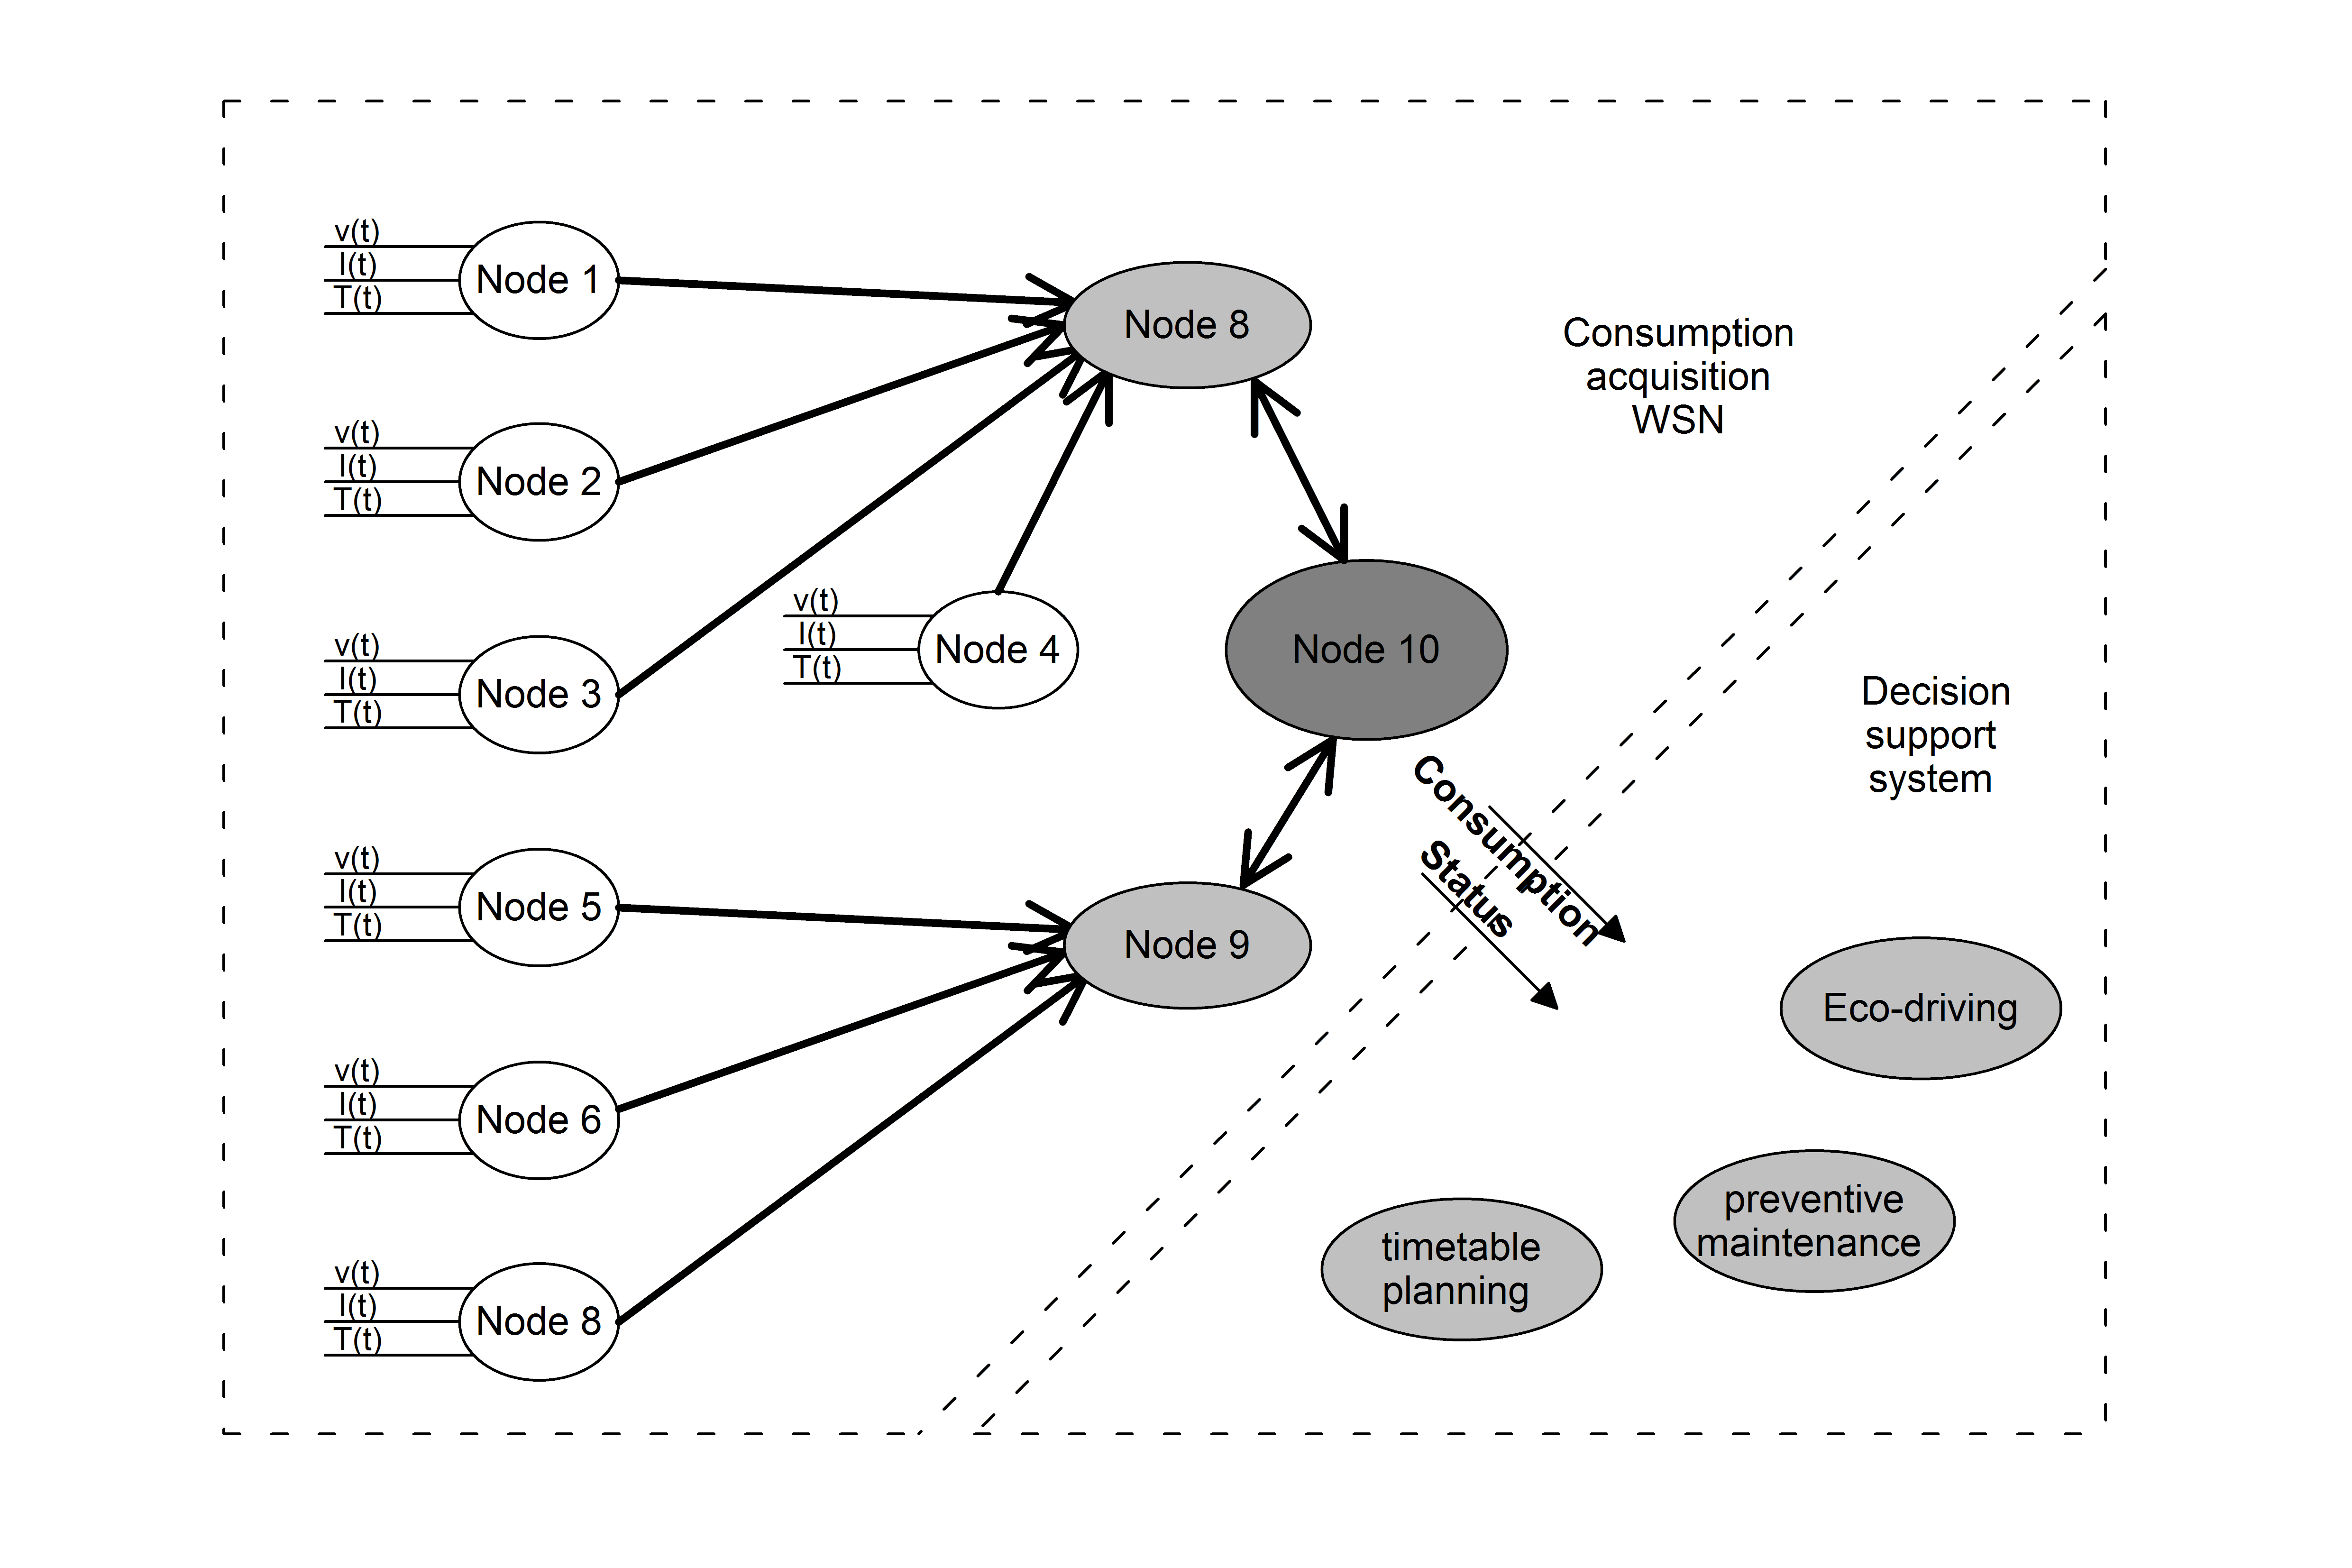
\includegraphics[width=0.75\textwidth,keepaspectratio]{figures/general}
	\caption{Integration of the WSN with a decision support system. }
	\label{fig:general}
\end{figure}

\newpage
Without an outlier detection mechanism, the decision support subsystem may have the following outputs:


\begin{description}
	\setlength\itemsep{-0.5em}
	\item[Input deviation from real value lower than a threshold]
	The Decision Support Subsystem output is according to the real consumption conditions.
	\item[Input deviation from real value greater than a threshold]
	The Decision Support Subsystem output is not according to the real consumption conditions.	
\end{description}

The problem of taking decisions based on wrong considerations of the consumption status may lead to loss in desirable efficiency or increase of costs.

Let us consider a simple and hypothetical example where the DSS will provide an output towards suggesting an action in preventive maintenance based on the usage of a component. Considering that the usage of the component is depending on the counting of situations that the component is working above the nominal conditions. Without an outlier detection mechanism, the outliers will induce the DSS to count situations of overcharge of the component where the measurement is not related to the working above the nominal conditions but is related to external influences such as EMI or temperature. The output of DSS may suggest a preventive maintenance on a component that is working in proper conditions.

To conclude, with an outlier detection mechanism in the consumption acquisition subsystem the decision support subsystem may know if the value of consumption is an outlier or not and, with that information, the DSS output will be more accurate with the real conditions of operation.

%%%%%%%%%%%%%%%%%%%%%
%%   Wireless sensor networks
%%%%%%%%%%%%%%%%%%%%%
\newpage
\section{Outlier detection in WSNs}
\label{sec:od_wsn}
Wireless sensor networks (WSNs) has been widely used in several applications in several domains such as industrial, scientific, medical and others. Those applications have been supported by the advances in wireless technologies as well as in the evolution of microcontroller technologies, with enhanced processing capabilities associated with reduced energy consumption.

\subsection{Motivation}

\cite{class:rajasegarar:2007} points an important motivation for the inclusion of computational algorithms, i.e. outlier detection algorithms, to reduce the transmission of erroneous data, since in WSNs, the majority of the energy consumption occurs in the radio communication. In particular, they present the case of Sensoria sensors and Berkeley motes where the energy consumption in communication exceeds in ranges from 1000 to 10000 the energy consumption of computation.

Thus, a research opportunity is raised to reduce the communication usage of $\mu C$s by adding processing features where the small increase in the computation will significantly reduce the energy consumption in the transmission. These processing features are, among others, the outlier detection algorithms.


On the field of the quality of the data acquired by WSNs, the motivation of detecting outliers in data acquired from WSNs has been extensively presented in the literature. The need for acquire data from harsh or "highly dynamic" environments as well as the need to validate and extract knowledge from the acquired data are one of the main points in the motivation to study the outlier detection in WSNs,  \cite{gen:zhang:2010,gen:chandola:2009,stat:ghorbel:2015,class:martins:2015b}.



\subsection{Research areas}
Zhang et al. \cite{gen:zhang:2010} identifies the outlier detection research areas in three domains: 

\begin{itemize}
	\item Intrusion detection: Situation caused by malicious attacks, where the detection techniques are query-driven techniques;
	
	\item Fault detection: Situation where the data suffer from noise and errors and where the detection techniques are data-driven ones;
	
	\item Event detection: Situation caused by the occurrence of one atomic or multiple events and where the majority of the research has been developed due to its complexity.
\end{itemize}

Based on the division of this three domains, the upcoming research is intended to be focused on the event detection and fault detection techniques. Specifically, the main goal for this research will be the event detection algorithms.


\subsection{Challenges}

The challenges of outlier detection in WSNs are related to the quality of the acquisition of the sensors, the reliability of the modules in terms of energy or environmental susceptibility, and the communication requirements and restrictions.

Zhang et al. \cite{gen:zhang:2010} lists the challenges as the following:

\begin{itemize}
	\setlength\itemsep{-0.5em}
	
	\item Resource constraints;
	
	\item High communication costs;
	
	\item Distributed streaming data;
	
	\item Dynamic network topology, \\ frequent communication failures, \\ mobility and heterogeneity of nodes;
	
	\item Large-scale deployment;
	
	\item Identifier outlier sources;
	
\end{itemize}

\cite{class:branch:2006} identifies an important challenge, where the probability of occurrence of outlier events are extremely small. \cite{nn:abid:2016} as well as \cite{stat:sheng:2007} identifies the large amount of data as the main challenge for outlier detection in WSN. \cite{nn:zhuang:2006} identifies the inexpensive and low fidelity sensors as the main reason for the error generation and, the main challenge are identified on the distributed streaming data among a large amount of sensors. \cite{stat:ghorbel:2015} points a main challenge as the processing of data from sensors that generates continuously data that is uncertain and unreliable. 

To conclude, and in the scope of the PhD, the main challenges will be the usage of inexpensive and low fidelity sensors that will be affected by the rush railway environment. Complementary, the main challenge of using outlier detection mechanisms in the railway WSN is the balance between the detection accuracy and the influence that undetected data-instances will induce in other subsystems (in particular in decision support systems dependent on data from the WSN). In addition, the detection accuracy is directly related with the memory usage, computational requirements, communication overhead, etc. 


\newpage

\section{Classification of outlier}
\label{sec:classint}
\cite{gen:zhang:2010} presents aspects to be used as metrics to compare characteristics of different outlier detection techniques. In parallel, \cite{gen:chandola:2009} presents a similar approach for the classification of outlier detection. 
In table \ref{table:t1} is present a comparison between two approaches to classify the nature of input sensor data.

	
%\input{tables/t1}
	

Based on the work of \cite{gen:zhang:2010} and \cite{gen:chandola:2009}, the table \ref{table:t2} identifies the different types of outliers. 
Those types differ on the objective of the outlier detection techniques: detect anomalies in individual data instances or in groups of data to detect irregularities, respectively, in local or in the global measuring system.

%\input{tables/t2}

\newpage


Table \ref{table:t3} continues the classification, focusing in three parts: 
\begin{itemize}
		\setlength\itemsep{-0.5em}
		\item The need of pre-classified data (to implement supervised, semi-supervised or unsupervised outlier detection techniques);
		
		\item The output of outlier detection techniques (binary labels for normal/abnormal data-set and a score for each data-set to evaluate the weight of being an anomaly)
		
		\item The identity of the outliers (detect errors, events or malicious attacks)
\end{itemize}

\newpage

%\input{tables/t3}

\vspace{2em}



\section{Taxonomy of Outlier Detection Techniques}
\label{sec:taxon}
The study of detection techniques requires a well-defined taxonomy framework that addresses the related work on the different areas. This taxonomy is well defined and solid in the literature, where the works of \cite{gen:zhang:2010} and \cite{gen:chandola:2009} reflect a similar approach on presenting a taxonomy for outlier detection techniques.

In the following sections a coverage in relevant techniques is presented:

\begin{itemize}
	\setlength\itemsep{-0.5em}
	\item Classification based techniques.
	\subitem Bayesian Networks
	\subitem Rule-based techniques
	\subitem Support Vector Machines
	
	\item Statistical based techniques.
	\subitem Parametric --- Gaussian based
	\subitem Non-parametric --- Histogram based
	\subitem Non-parametric --- Kernel function based
	
	\item Nearest Neighbor-based techniques.
	\subitem Using distance
	\subitem Using relative density
	
	\item Clustering based techniques.
	
	\item Spectral Decomposition based techniques.
	
\end{itemize}


%%%o resto deste capítulo está dividido em ficheiros












\chapter{Future Research}
%\lipsum[4-4]
In this chapter there are presented the future steps in research on outliers detection on railways WSN-based smart grid.


%%%%%%%%%%%%%%%%%%%%%
%%   Smart metering Systems
%%%%%%%%%%%%%%%%%%%%%
\section{Outliers detection definition}

\lipsum[1]


\section{Synthesis}

\chapter{Conclusion}
%\lipsum[1]

With this work, we propose and implement a solution for the wireless monitoring of power converters. The main challenge of this wireless monitoring is to obtain energy data of a system in a harsh environment. The motivation for this work is to study the implementation of a wireless monitoring system in railway environment, based on the outcomes of the implementation of such monitoring system in a renewable energy generation system.

The system specification was defined, with the construction of a System Requirement Specification (SRS) document as the main outcome. In addition, it was performed an overview on existing wireless communication systems, a market survey on available technologies, and the protocols, standards and communication KPI's was raised.

A specific technology was selected, on the family of wireless MCU's. The implementation stage complies with the definition of the hardware and software architecture. The communication results validates the acquisition of electric measurements from multiple PV power converters. 

The lack of data results is clear. Any of the communication KPI's was not evaluated due to the need of further development. This further development depends on a new solution for the interface between the power converter and the wireless node, since the communication link is highly affected by the noise of power converter.

For future work is clear the need of evaluating all the proposed communication KPI's. This task requires a new electronic board to interface the remote node. Complementary, the data concentrator should be improved to implement a local database and a serial request-response protocol to exchange data with the microgeneration system master.

We conclude that the methodology followed and the proposed solution validates the objective of this work, which is the wireless monitoring of a power converter.



\bibliographystyle{chicago}
%chicago}

\bibliography{outliers,shift2rail,references}
%\bibliography{outliers}
%\PrintBib{outliers, }


%\bibliographystyle{plainnat}
%\bibliography{references}


\end{document}